\section{Issue Handling Management}
In the event of issues with the solution the three steps in figure \ref{fig:issue_handling} must be obeyed. The steps will help to resolve the incident in a generic fashion and reach an appropriate solution.

\begin{center}
\begin{figure}[H]
\centering
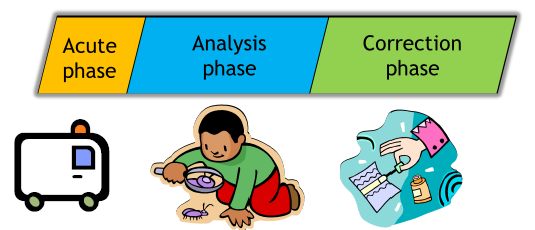
\includegraphics[width=0.95\textwidth]
{Billeder/IssueHandling.PNG}
\caption{Issue Handling}
\label{fig:issue_handling}
\end{figure}
\end{center}

\subsection{Acute Phase}
When the incident is perceived it is important to stop the issue from escalating. Then the relevant personnel must be informed of the issue and necessary workarounds must be made.
This phase is also where evidence of why the issue happened is secured for later analysis.

\subsection{Analysis Phase}
The issue must be identified and described. Find out what circumstances and activities led up to the incident. It is important to discern between the cause and the effect of the incident. The extent of the issue has to be evaluated and the affected customers must be handled. The consequences must be assessed and corrections must be decided and approved.

\subsection{Correction Phase}
The correction of the issue may involve changes to the system and new training of people. The customer may have different needs, requirements and opinions on how to resolve the issue.

\subsection{Example of specific issue handling}
This is an example of an issue in the system. The issue takes base in the identified risk no. 8 in table \ref{table_risks}: Hardware breaks. If some of the hardware in the system breaks it will have dire consequences for the use and the users.

In this example the hardware running the hand-held dismounted COP is broken. The first thing to do is to extract the affected user, since he might vulnerable without the COP. While extracting the user evidence of the problem must be secured. The issue is reported to the support team, who will start the investigation of the issue.
The support team will identify and describe the broken device and find the root cause of the problem. The support team will discuss if the hardware can be repaired or has to be replace. If design failures is discovered in the product, the design should be subject for design changes. In the Correction Phase the accepted solution from the analysis is carried out. If the changes affect the user experience the users have to be informed and trained accordingly.